\documentclass[UTF8]{ctexart}
\usepackage{geometry}
\geometry{left=2.0cm,right=2.0cm,top=2.5cm,bottom=2.5cm}
\usepackage{amsmath}
\usepackage{amsthm}
\CTEXsetup[format={\large\bfseries\heiti\textbf}]{section}
\usepackage{subfigure}
\usepackage[graphicx]{realboxes}
\usepackage{caption}


\title{平面图顶点覆盖问题报告}
\author{孟悦琦}

\begin{document}
\maketitle

\section{背景介绍}
在计算理论研究过程中,NP完全问题是十分重要的一类问题。
若语言$L$是NP完全问题,应满足:1. $L$是NP问题。 
2. 对于每一个NP问题$L'$,存在一个多项式时间内的规约,使得$L'$规约到$L$。
像我们熟知的SAT问题,独立集问题(IS)都NP完全问题。顶点覆盖问题也是一类NP完全问题。
并且,对于定点覆盖问题,若加以平面图的条件限制,以及最大顶点度为3的条件限制后,仍然可以证明其是NP完全问题。
以下给出详细证明:

\section{平面图顶点覆盖NP完全性证明}
在证明过程中,使用了一关键结构。此结构如图1.1所示。
\begin{figure}[htbp]
    \centering %表示居中
    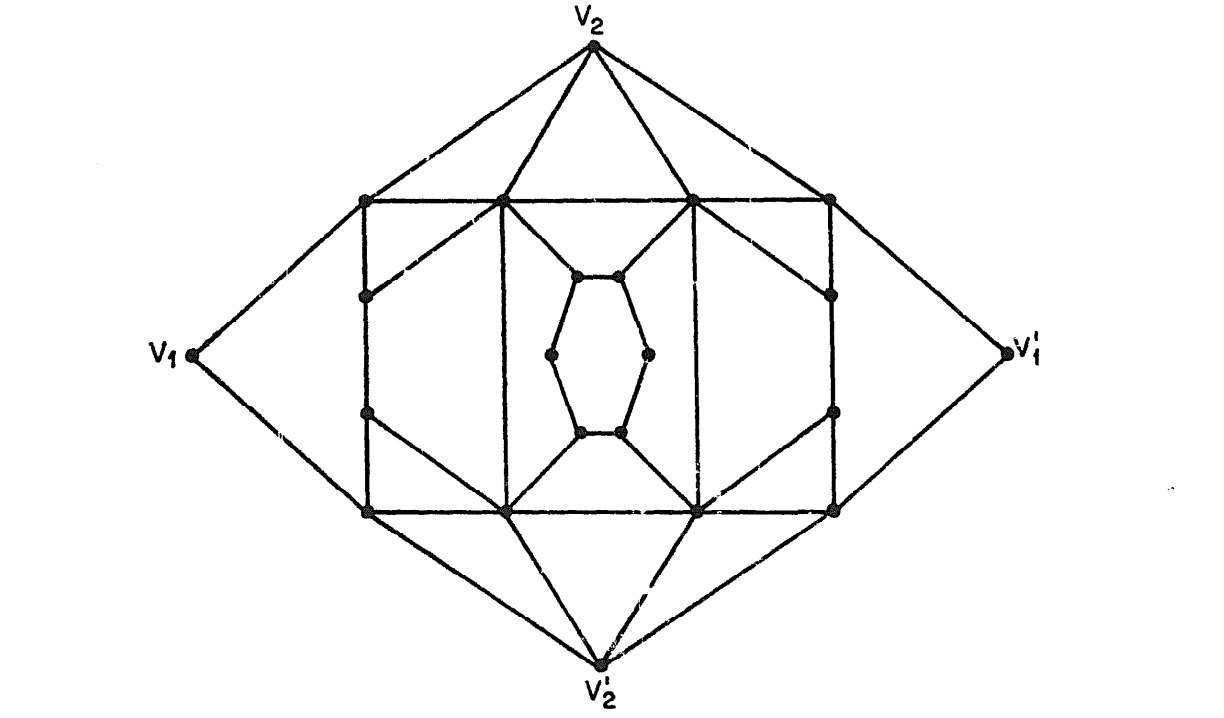
\includegraphics[height=4.5cm]{graph1.png}
    \caption{交叉($crossover$)结构}
    %图片的名称
    % \label{2}
    %图片的标签,用于文章中的引用,注意到标签的数字与实际文章显示的数字可能不同
\end{figure}
该结构可以被命名为交叉结构($crossover$),它的四个出口位置被标记为$v_1,v_2,v_1',v_2'$。
对于任意$i, j$,满足$0 \leq i,j \leq 2$,那么,令 $c[i,j]$ 表示所有顶点覆盖C的最小基数,顶点覆盖满足如下条件:
\begin{gather*}
    |\{V_1, V_1'\} \cap C| = i \And 
    |\{V_2, V_2'\} \cap C| = j
\end{gather*}
通过观察交叉结构,我们发现,当$i=1$或$j=1$时,$c[i,j]$的值和选取哪一个出口顶点无关。
表1中给出了所有$i,j$取值下,$c[i,j]$的值。通过观察表1,我们发现如下性质:对于$0 \leq l \leq 2$,有:
\begin{gather*}
    {\rm (A)} \quad c[1,l] - c[0,l] \leq 1 \And c[l,1] - c[l,0] \leq 0 \\
    {\rm (B)} \quad c[2,l] - c[1,l] =  c[l,2] - c[l,1] = 1
\end{gather*}
\begin{figure}[htbp]
    \centering %表示居中
    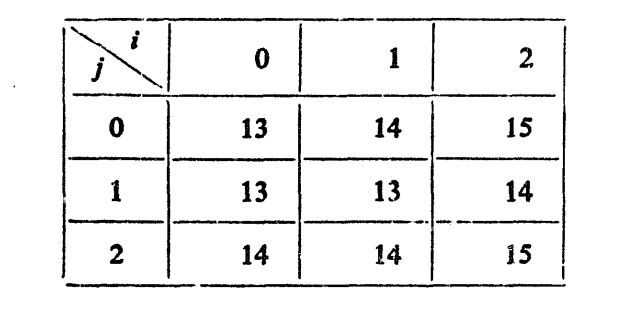
\includegraphics[height=4.5cm]{table1.png}
    \caption*{表1:所有可能的$c[i,j]$值}
    %图片的名称
    % \label{2}
    %图片的标签,用于文章中的引用,注意到标签的数字与实际文章显示的数字可能不同
\end{figure}
\par
对于给定的一个图$G=(N,A)$,我们可以进行如下变换,生成新图$G'=(N',A')$。
使用交叉($crossover$)结构变换,具体方法如下:\par
1. 将图$G$在一个平面中表示,允许边之间存在交叉。 \par
2. 对图中的每个交叉点,用交叉($crossover$)结构代替。\par
\noindent 具体替代过程如下图所示:
\begin{figure}[htbp]
    \centering %表示居中
    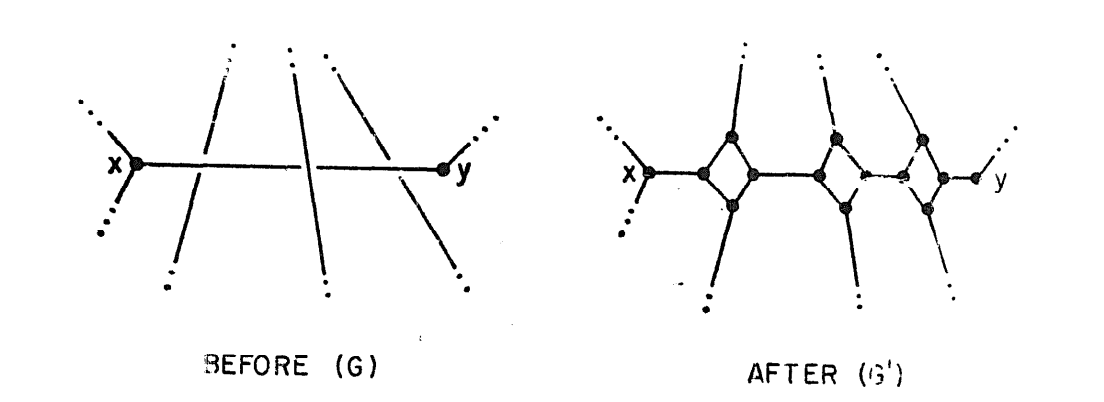
\includegraphics[height=4.5cm]{graph2.png}
    \caption{代替过程}
    %图片的名称
    % \label{2}
\end{figure}

使用交叉结构来替代$\{x,y\}$上的交点,这些交叉结构可以被称作是$\{x,y\}-line$上的交叉结构。
连接$\{x,y\}-line$上交叉结构与$x,y$的,为$\{x,y\}-line$上的边。
$\{x,y\}$是$\{x,y\}-line$上的结点。临近$x$结点的交叉结构出口被称作$y$出口,临近$y$的被称作$x$出口。 \par

我们令$d$是图$G'$中使用交叉($crossover$)结构的数量。
显然,$G'$中的边可以被分为两部分:(1)在$\{x,y\}-line$上的边。(2)在$d$个交叉结构上的边。
通过使用顶点集合$x$和每个交叉结构的$x$出口或$y$和每个交叉结构的$y$出口,所有$\{x,y\}-line$上的边可以被覆盖。
而交叉结构中的边仅能使用交叉结构内部的结点进行覆盖。
经过之前所描述的变换,$G$中的所有边的交点,在$G'$中都被交叉结构所取代,因此,$G'$是一个平面图。
并且,由于$n$个顶点至多有$O(n^2)$条边,至多有$O(n^4)$个交点,显然这个规约可以在$poly(n)$时间内完成。
于是我们只需要证明,对于任意$k$,图$G$有一个大小为$k$的顶点覆盖当且仅当图$G'$有一个大小为$k+13d$的顶点覆盖。 \par

首先,我们假设$S$是图$G=(N,A)$的顶点覆盖,并且$|S|=k$。我们用如下方法对$G'$的顶点覆盖集进行构造。
对于任意边$\{x,y\} \in A$,令$f(x,y)$为在$S$中的$xy$的端点。构造集合:
\begin{gather*}
    S' = \{v: \mbox{对于}\{x,y\} \in A, v\mbox{为}\{x,y\}-line\mbox{上交叉结构的}f(x,y)\mbox{出口} \}
\end{gather*}
由于$S$是$G$中的一个顶点覆盖,$f(x,y)$包含了所有$A$中的边,于是有$S \cup S'$可以覆盖所有非交叉结构中的边。
同时,由于每一个交叉结构在$S'$中被计算了两次,故有$|S'|=2d$。之后要完成的便是覆盖交叉结构中未被覆盖的边。
这是我们观察表1,由于每个交叉结构,每对出口都被覆盖了一次,那么由于$c[i,j]=13$,我们只需在每个交叉结构中添加11条边即可。
令$S''$为每个交叉结构需要添加的11条边组成的集合。
那么$S \cup S' \cup S''$即为$G'$的顶点覆盖,同时有$|S \cup S' \cup S''|=k+2d+11d=k+13d$,满足规约假设。 \par

相反的,我们假设$G'$中存在一个基数为$k+13d$的顶点覆盖。令:
\begin{gather*}
    k^* = {\rm min}\{|S|:S\mbox{是}G'\mbox{的顶点覆盖}\} \\
    M = \{S: S \mbox{是}G'\mbox{中的一个顶点覆盖,且}|S|=k^*\}
\end{gather*}
对于每一个$S \in M$,我们定义:
\begin{gather*}
    m(S) = |\{x \in S : x \mbox{是} G' \mbox{中交叉结构的出口结点}\}| \\
    m^* = {\rm min}\{m(S):m(S) \in M\}
\end{gather*}
这时,令$S^* \in M$表示一个符合条件$m(S^*)=m^*$的顶点覆盖。
根据表1,由于至少在每个交叉结构中有13个结点,我们可以得到$|S^* \cap N| \leq k$。
于是我们仅需要证明$S' = S^* \cap N$是图$G$的一个顶点覆盖。 \par
我们使用反证法证明。假设不是,那么存在$\{x,y\} \in A$有$S' \cap \{x,y\} = \phi$,因此$s^* \cap \{x,y\} = \phi$。
我们令$l$时$\{x,y\}-line$上的交叉结构数量。由于有$l+1$条边在$\{x,y\}-line$上,故必须有至少$l+1$个顶点在$S^*$中,且由于$x,y$都不再其中,这$l+1$个顶点应都是交叉结构的出口。
如果我们令$n(i)$为$\{x,y\}-line$中有$i$个交叉结构出口在$S^*$中的数量,那么有$n(2)-n(0) \geq 1$,我们证明这样会产生矛盾。 \par
我们令$X_i$为$\{x,y\}-line$上的第$i$个交叉结构的全部结点,有$1 \leq i \leq l$,令$S_i = X_i \cap S^*$。
令$T_i \subseteq X_i$为一个包含$x$出口和$S_i$中非出口结点的顶点覆盖,$X_i$在包含这些顶点的同时,具有最小基数。
对每一个$i$,$r(i)$为$S_i$中第$i$个交叉结构出口的个数。根据之前的(A)与(B),得到:
\begin{align*}
    & r(i) = 0\mbox{时} \quad |T_i| \leq |S_i| + 1 \\
    & r(i) = 1\mbox{时} \quad |T_i| \leq |S_i| \\
    & r(i) = 2\mbox{时} \quad |T_i| \leq |S_i| - 1 \\
\end{align*}
令$T_i = \bigcup_{i=1}^{l} T_i $,$S_i = \bigcup_{i=1}^{l} S_i $。由于$n(2)-n(0) \geq 1$,我们得到:
\begin{gather*}
    |T| \leq |S| - 1
\end{gather*}
同时,根据之前的定义我们发现,$T$至少比$S$少一个交叉结构的出口顶点,同时有相同数量的交叉结构非出口顶点。
同时我们发现,$T \cup {x}$可以覆盖所有$S$覆盖的非交叉结构上的边。
于是$T^* = (S-S^*) \cup T \cup {x}$是$G'$的顶点覆盖。同时:
\begin{gather*}
    |T^*| = |S| - |S^*| + |T| + 1 \\
    m(T^*) = m(S^*) - 1 = m^* - 1
\end{gather*}
这与$m^*$的定义相矛盾,于是有$S^* \cap N$为$G$的一个顶点覆盖。 \par
于是证明顶点覆盖问题在$poly(n)$时间内规约到平面图顶点覆盖问题的正确性。$\qedsymbol$ \par
需要注意的是,当输入图$G$的顶点度不超过3时,生成的图$G'$的顶点度不会超过6。
这说明对于顶点度最多为6的平面图来说,其顶点覆盖问题是一个NP完全问题。

\section{最大顶点度为3平面图顶点覆盖NP完全性证明}
首先,由于顶点覆盖问题是NP问题,并且最大度数为3的平面图顶点覆盖问题亦为顶点覆盖问题,故此问题存在非确定图灵机$poly(n)$时间内求解的算法。
即有最大顶点度数为3的平面图顶点覆盖问题为NP问题。 \par
给出一个平面图$G$和它的顶点覆盖集基数$k$,我们构造一个平面图$G'$,$G'$满足最大顶点度为3。
同时构造$k'$为$G'$中的顶点覆盖集的基数。
我们只需要证明$G'$有一个大小为$k'$的顶点覆盖集合,当且仅当$G$有一个大小为$k$的顶点覆盖集合。\par
假设图$G=(V,E)$,其中$V=\{v_1,v_2,\dots,v_n\}$。我们从$G=G_0$开始进行迭代变换。
对于每一个整数$i$,图$G_i$可以通过图$G_{i-1}$变换得来。具体方式如下: \par
1. 令$\{v_i,w_1\},\{v_i,w_2\},\dots,\{v_i,w_p\}$,为图$G_{i-1}$中与$v_i$连接的边,且按照顺时针顺序。 \par
2. 将$v_i$替换为新结点组$u_i(j),v_i(j)$,其中$1 \leq j \leq n$,且存在边$\{u_i(j),v_i(j)\}, 1 \leq j \leq n$,$\{v_i(j),u_i(j+1)\}, 1 \leq j \leq n-1$,以及$\{v_i(n),u_i(1)\}$。 \par
3. 去除所有边$\{v_i, w_j\}$,添加边$\{v_i(j), w_j\}$,增加一个顶点$z_i$,增加边$\{u_i(1),z_i\}$ \par
\begin{figure}[htbp]
    \centering %表示居中
    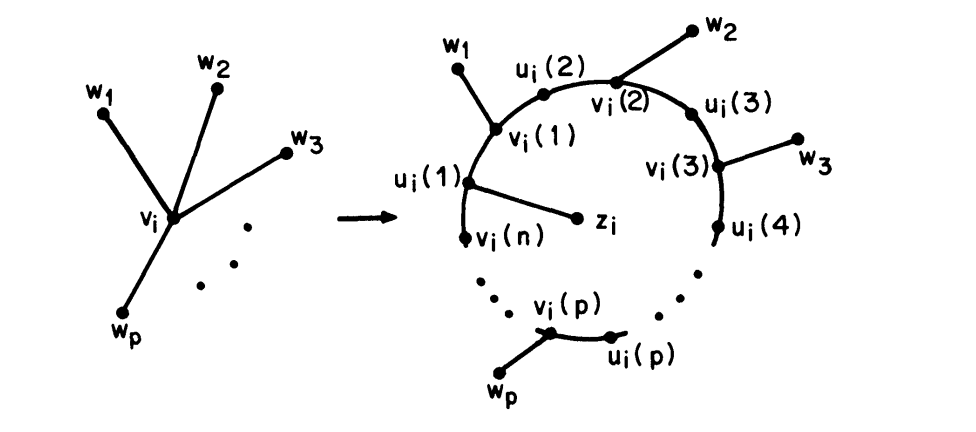
\includegraphics[height=4.5cm]{graph3.png}
    \caption{变换过程}
    %图片的名称
    % \label{2}
\end{figure}
\noindent 于是我们令$G'=G_n$,$k' = n^2 + k$。显然$G'$中没有顶点度超过3。 \par
下面我们假设顶点集$V^*$为图$G$的一个基数至多为$k$的顶点覆盖,我们构造图$G'$的基数不大于$k'$顶点覆盖集$V_1^*$,构造方式如下:
\begin{gather*}
    V_1^* = \{v_i(j): v_i \in V^*, 1 \leq j \leq n\} \cup \{u_i(1): v_i \in V^*\} \cup \{u_i(j):v_i \notin V^*, 1 \leq j \leq n \}
\end{gather*}
经过计算得出,$|V_1^*|=nk+k+n(n-k)=n^2+k=k'$。
由于顶点数量是$O(n^2)$的,故必定可以在$poly(n)$的时间内完成规约的过程。
于是我们只需证明$V^*$是$G$的顶点覆盖,当且仅当$V_1^*$是$G'$的顶点覆盖。 \par
首先,若$V^*$为$G$的顶点覆盖,那么显然$u_i(1),1 \leq i \leq n$在集合$V_1^*$中。
故边$\{u_i(1),z_i\}$必定被覆盖。
且根据$V_1^*$中的元素构成,边$\{u_i(j),v_i(j)\}, 1 \leq j \leq n$,$\{v_i(j),u_i(j+1)\}, 1 \leq j \leq n-1$,以及$\{v_i(n),u_i(1)\}$亦必然被覆盖。
而对于边$\{v_i,w_t\}$,使用反证法。
若$V_1^*$中不存在覆盖边$\{v_i(j),w_t\}$的顶点,那么有$v_i(j) \notin V_1^* \And w_t \notin V_1^*$。
设$w_t \in \{v_k(s): 1 \leq k,s \leq n, k \neq i\}$。
那么显然有$v_i \notin V^* \And v_k \notin V^*$。
那么,对于$V^*$,必有一条边$\{v_i,v_k\}$未被覆盖,这与$V^*$的定义矛盾。 \par

相反的,假设$V_1^*$是$G'$的一个顶点覆盖,满足$|V^*| \leq k'$。
那么由于覆盖$G$中对应边的顶点是$G'$中的顶点,故构造:
\begin{gather*}
    V^* = \{v_i: \mbox{对于}j,1 \leq j \leq n,v_i(j) \in V^*_1\}
\end{gather*}
显然$V^*$必定是$G$的顶点覆盖。我们只需证明$|V^*| \leq k$。
首先,我们可以假定$u_i(1) \in V_1^*$,这是因为边$\{u_i(1),z_i\}$必定被覆盖且$z_1$的度为1。
对于$1 \leq i \leq n$,定义$S_i$:
\begin{gather*}
    S_i = V_1^* \cap \{u_i(j),v_i(j):1 \leq j \leq n\}
\end{gather*}
为了覆盖$v_i$环上的$2n$个顶点,我们必定有$S_i \geq n$。
由于$k' = n^2+k$,这意味着最多有$k$个$i$满足$S_i \geq n$。
更进一步,由于$u_i(1) \in S_i$,基数为$n$的$S_i$必定为$\{u_i(j): 1 \leq j \leq n\}$。
所以如果有$|S_i| > n$,则存在$v_i(j) \in S_i$。
由于此种情况最多出现$k$次,于是得到$|V^*| \leq k$,$V^*$是符合要求的图$G$顶点覆盖集。 $\qedsymbol$ \par
由此我们证明了对于顶点最大度为3的平面图,顶点覆盖问题也是NP完全问题。

\section{总结}
本篇本文章主要讲述了NP完全问题中的平面图顶点覆盖问题,并给出了详细证明。
对于平面图的顶点覆盖问题,当给予限制条件顶点度最大为3时,此问题仍为NP完全。



\end{document}
